%% *************************************************************************
%%
%% This is the PDD for the Rovers Study - Fall 2018
%%
%% This document uses IEEEtran.cls, the official IEEE LaTeX class
%% for authors of the Institute of Electrical and Electronics Engineers
%% (IEEE) Transactions journals and conferences.
%%
%% *************************************************************************

%% *************************************************************************
% LaTeX REFERENCES
% ----------------
%   Intro to LaTeX: http://www.rpi.edu/dept/arc/docs/latex/latex-intro.pdf
%   Comprehensive LaTeX symbol list: http://tug.ctan.org/info/symbols/comprehensive/symbols-a4.pdf
%% *************************************************************************

% tell \LaTeX what kind of formatting to use
\documentclass[conference]{IEEEtran} % http://www.ctan.org/pkg/ieeetran
\usepackage{blindtext} % enable placeholder text generator
\usepackage{graphicx} % enable toolbox for embedding figures and pictures
\usepackage{nomencl} % enable package for adding a list of variables and constants at the beginning, aka "nomenclature"
\usepackage{siunitx} % enable package for easily formatting units
\usepackage{hyperref} % enable package for cross-referencing figures, sections, references etc.
% how to use hyperref: http://www2.washjeff.edu/users/rhigginbottom/latex/resources/lecture09.pdf
\usepackage[T1]{fontenc} % change text encoding to make it more crisp
\usepackage{etoolbox} % enable conditionals for help text
\usepackage{booktabs} % make beautiful tables!

% initialize nomenclature package
\makenomenclature{}

% set title. choose something as descriptive and precise as possible. Descriptive > sounding cool. remember this!
\title{RIT Space Exploration Project Design Document Standard Format and Sample Content}


\author{
  % List the authors of the design document. 
  \IEEEauthorblockN{% This block is for author Names.
    Thomas~Hall\IEEEauthorrefmark{1}
  }
  \IEEEauthorblockA{% This block is for the author Affiliations, aka department and university
    RIT Space Exploration, Rochester Institute of Technology \\ %\\ starts a new line
    Rochester, N.Y. \\
    Email:
    \IEEEauthorrefmark{1}tjh2822@g.rit.edu
  }
}

% page header for pages other than cover page
\markboth{Project Design Document Standard}%
{Hall \MakeLowercase{\textit{et al.}}: RIT Space Exploration}

% Initial setup is over, start building the document itself
\begin{document}
\maketitle%
% correct bad hyphenation here, separated by spaces
\hyphenation{explor-ation}

\begin{abstract}
  Conduct a feasibility study on the design and construction of a self driving rover. A rover would be an area of space exploration completely new to SPEX, because of this there are a lot of unknowns that need to be answered before starting this project. The study would look at the talent and skills of RIT Space Exploration and answer the question: what caliber of rover are we able to make. It would employ a multidisciplinary team to cover for construction and development. The study would lean directly into a rover project in the future. The rover would be extremely promotable and would look great at Imagine RIT. 
      % The abstract is a brief summary of the design document. Typically it includes the purpose of the design document, key goals or objectives, and justifications.
\end{abstract}

\label{sec:nomenclature}
\newcommand{\nomunit}[1]{%
\renewcommand{\nomentryend}{\hspace*{\fill}#1}}
\renewcommand{\nompreamble}{}

\nomenclature{RIT}{Rochester Institute of Technology}
\nomenclature{SPEX}{RIT Space Exploration}
\nomenclature{PDD}{Project Design Document}
% Below are examples of using nomenclature for math symbols and constants or units
\nomenclature{$\dot{m}$}{Mass flow rate
  \nomunit{\,\si{\kilo\gram\per\second}}}
\nomenclature{$c$}{Speed of light
 \nomunit{\,\SI{2.9979e8}{\meter\per\second}}}
\printnomenclature{}

% The sections included here are required. Additional sections and subsections may be added as necessary.
\section{Introduction}
\label{sec:introduction}
  % The introduction is a place to give background and context before diving into the subject matter.
  % Establish context for the work you are about to propose and the main ideas of the proposition itself.

\IEEEPARstart{R}{obotics} and by extension rovers are a tremendously important part of space exploration. 
This is also an area that RIT Space Exploration has very little experience with project-wise. 
The purpose of this study is to assess and assert the capability of RIT SPEX in regard to the construction and fabrication of a mock-rover. 
As this is a new area to RIT SPEX a study is necessary to most effectively accomplish this goal. 
This study will look at the unknowns, technical challenges, project management, and member skills of RIT Space Exploration.
The study is intended to last exactly 1 semester with the deliverable of a PDD of the following semester where the team would shift focus from design and research to fabrication and testing. 

\section{Primary Objective}
\label{sec:primary-obj}
  % At the end of the day, whether the project ``succeeds'' or ``fails'' is judged against the objectives it sought to meet.
  % Note that results that contradict expectations/hypotheses are not failures if the scientific \& engineering methods are followed along the way.
  % Sometimes our expectations are wrong and that can be just as successful as getting data we thought we'd see.
  % What matters are what questions you intend to answer.
  % This is the main purpose or main goal the project hopes to achieve.

The goal of this study is to asses the technical ability and skills of RIT Space Exploration regarding the construction and implementation of a mock rover. 
This study will create a plan including answering unknowns about the rover, how the rover will be built and programmed, and what skills / resources are needed to build the aforementioned rover. 

At the end of the semester these questions will lead to a well-developed PDD for the following semester.  

%\begin{figure}
%  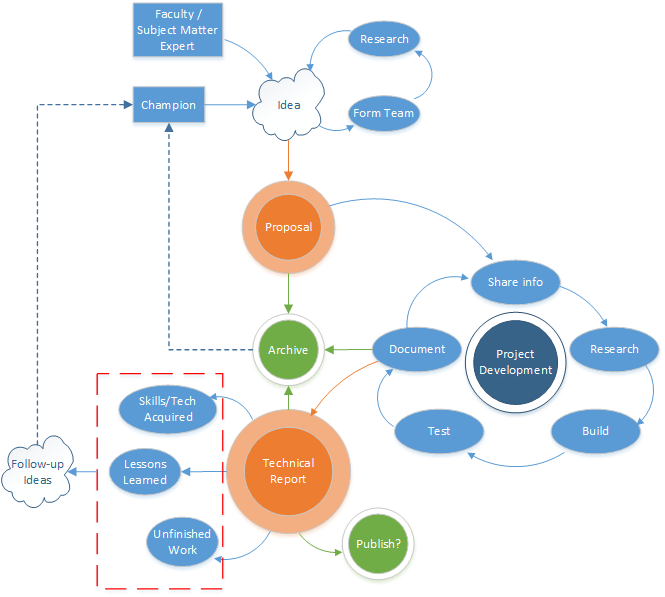
\includegraphics[width=\linewidth]{figs/project-life-cycle.png}
%  \caption{A PDD is the first piece of documentation to be archived in the project life cycle. Since the life cycle can be iterative, a new design document may also refer to one or more previous SPPs.}
%\label{fig:lifecycle}
%\end{figure}

\section{Secondary Objectives}
\label{sec:secondary-obj}
  % Secondary Objectives are lower priority or bonus objectives that are significant but not the main focus of the project. This template does not have secondary objectives.
The study will also investigate the University Rover Competition (URC) as hosted by the mars Society as a potential long term goal. The competition is held annually and features 4 very intense competitions. Such a rover would need to be fully self navigating, perform scientific analysis on soil samples, and having a robotic arm capable of fine motor control. Such a project would be among the most ambitious SPEX has ever attempted. 

\autoref{tab:questions} lists questions the project will need to answer in order to make a PDD.

\begin{table*}
% this table is too wide for the two-column format, so we let it expand across both columns
% we haven't told LaTeX where to put this so it'll find the best place.
    \caption{List of questions study will answer}
    \centering
    \begin{tabular}{@{}llcc@{}}
        % READ THIS!! https://www.inf.ethz.ch/personal/markusp/teaching/guides/guide-tables.pdf
        \toprule % line on top external edge of table
        % Separate cells in a row with &, move to the next row with \\
        Question & Area \\
        \midrule % line separating two internal rows
        Will the rover design be based on something else? If so, what design? & General \\
        What hardware will be present on the rover? (Electronics + Structure) & Hardware \\
        What type of software will be on the rover & Software \\
        What libraries (if any) will the software be utilizing? & Software \\ 
        How will the rover navigate terrain? & Navigation \\
        Will the rover (ever) be self-driving? If so, how will this be accomplished? & General \\
        What will power the rover? & Electrical \\
        How much will the rover cost? & Hardware \\
        How will the rover be funded? & General \\
        What drive terrain will the rover feature? & Locomotion \\
        Will the rover feature any kind of robotic arm? & Hardware \\
        How will the rover hardware be tested? & Testing \\
        How will the rover software be tested & Testing \\
        Is the University Rover Challenge a possibility in the future? What steps can be taken to participate? & Competition \\
        How will the wheels/treads work? & Hardware \\
        What suspension system (if any) will the rover feature? & Hardware \\
        How can the rover be improved in the future? & General \\
        How can this project be broken up into smaller sub projects / teams? & General \\
        What are the next logical steps for the rover? (i.e. what work can be done in future semesters?) & General \\
        What will the team aim to have present at ImagineRIT 2019? & General \\ 
        Will the rover feature and special scientific equipment? (Drill, soil, etc...) & Hardware \\
        Do any areas of the rover design overlap with other SPEX areas? What about other clubs at RIT? & General \\
        To what spec will the rover be built? & Hardware \\
        Could RIT SPEX partner with another organization for the URC & Competition \\
        What are the navigation goals for this rover? (What gradient incline, etc...) & General \\
        What elements of the URC competition should this rover be built to do? & General \\
        What are the dimensions of this rover? & General \\
        % LaTeX doesn't really like multi-line cell contents. Try to keep the text in each cell concise!
        \bottomrule
    \end{tabular}
\label{tab:questions}
\end{table*}

\section{Benefit to SPEX}
\label{sec:benefit}
% Explains the benefit to RIT SPEX

Rovers are a huge part of space exploration. It is also an area that SPEX is not currently involved with. 
It would be beneficial to our members to get some experience in this area.
A rover would look super good for SPEX at Imagine RIT. 
The rover would be rather large and would attract many eyes. We could even demo it outside if there is sufficient space. 
A rover would be very easy to get video and photos of for SPEX promotions. 
Having a rover is also another opportunity for SPEX to fundraise. 
There is plenty of space to place company logos on the body of the rover. It would also allow for SPEX to reach out to robotics companies.. 
The self driving component would be the heaviest computer science project SPEX would have attempted. 
This would help with retention of CS and SE majors. 
Machine learning and artificial intelligence are at the forefront of computer science right now. 
They are heavily desired in industry including space exploration.
This study would figure out the capabilities of SPEX in regards to this goal. 
It will also eliminate many of the unknowns and answer many of the questions at the start of a project like this. 
This study will create a rough plan for building such a rover.



% Subsections

\subsection{Mindset}
\label{subsec:mindset}
The purpose of this study is to eliminate unknown for a potential rover project. 
Because of this the team members must be in the mindset to analyze each part of the project and identify as many problem areas that need answers as possible. 
This means being specific on how we are going to accomplish our goals. 
What material, what algorithm, with what method will we be accomplishing this.

\subsection{Traceability}
\label{subsec:traceability}

It is important that the team members document the sources they use to gather information. 
There will be a Google Drive folder that will hold notes with links to any books, articles, media or their sources that are relevant to the rover project. 

\subsection{Assessing Technical Skills}
\label{subsec:assessing-technical-skills}

Building a rover, especially one built to URC specifications requires a large team with a diverse set of technical skills. 
This study will look at RIT SPEX and asses what areas are sufficient and what areas need to be developed in order to build a rover. 
It will also let us know to what spec we are currently capable of building such a rover. 

\subsection{Accessibility}
\label{subsec:plug-n-play}

The study would require a handful (4-5) members each with different areas of expertise. The members would need that knowledge as well as \LaTeX{}, notetaking, and good research practices.

\section{Implementation}
\label{sec:implementation}
  % What path do you anticipate the project to take?

This project would involve divvying out the different project areas to the different team members and each week meeting to discuss progress. 
The team would take this information, refine it and put it into the PDD draft. 
Approx. 10 weeks into the semester the mechanical team should be able to build a rough CAD model and do any prototyping.
The PDD would be finished by the end of the semester (or earlier) and the project would be free to shift to second semester work.    

\subsection{Deliverables}
\label{subsec:deliverables}
  % When all is said and done, what will you have to show for it?
  % Examples: Hardware, software, poster, ImagineRIT demo, presentations, technical papers...
The primary deliverable of this study will be a PDD for the spring. It is also noted that the materials that the team will come across or notes should also be saved in an Google Drive folder for future reference.  
The team will also present at SPEX design reviews and the weekly checkups at general meetings with the areas the team members are studying that week.
The should have a rough CAD model for the PDD showing the spacing and layout of the potential rover. 
The team may decide to use said CAD model to prototype. 

\subsection{Milestones}
\label{subsec:milestones}
  % Be as detailed as you can, but it's okay if there are unknowns.
  % At the very least, specify how many semester you expect the project to take until it reaches completion.
The largest milestones would be PDD draft and completion. This can also be expanded to include the CAD models and any prototypes. 

\section{Externalities}
  % Things not directly related to the work or outcomes, but related to the project as a whole.
\subsection{Prerequisite Skills}
  % Which skills do team members need to have before work can start (not including skills that will be learned ``on the job'')?
The study is going to require members that are knowledgeable in mechanical design and manufacturing, software engineering, machine learning, electrical engineering, and project management. These members will also need to be experienced in research and design document work. Though this seems simple, finding SPEX members to do this well  

\subsection{Funding Requirements}
  % Estimate costs that would be needed to meet objectives.

The cost of this study is relatively minimal as it is a study. 
There may be physical prototype costs but these should again be very small. 
Physical prototyping can be done with cheap materials like cardboard or foam core.  

\subsection{Faculty Support}
  % Identify faculty that will be involved (or would need to be involved) to meet objectives.
  % Note that if a professor is the Principal Investigator (P.I.) for a project, there still needs to be a student as the SPEX Project Champion.
Support from faculty could greatly advance this study and what RIT SPEX is capable robotics wise. The team should reach out to professors for advice and help.

\subsection{Long-Term Vision}
\label{sec:vision}
The long-term vision of this project is to open RIT Space Exploration up to a new area of projects and development. Robotics and rovers are at the core of deep space exploration and most science missions. The University Rover challenge is also a worthy long term goal. 

\section*{Acknowledgements}
The author would like to thank SPEX alumni Phil Linden for creating the PDD template, Anthony Hennig for founding RIT Space Exploration, and all the SPEX members that continue to invest their time and energy into the pursuit of space exploration.

\bibliographystyle{IEEEtran}
\bibliography{sample-with-examples}

\onecolumn
\appendices{}
%\section{Project Life Cycle}
%\begin{figure}[h]
%  \centering
%  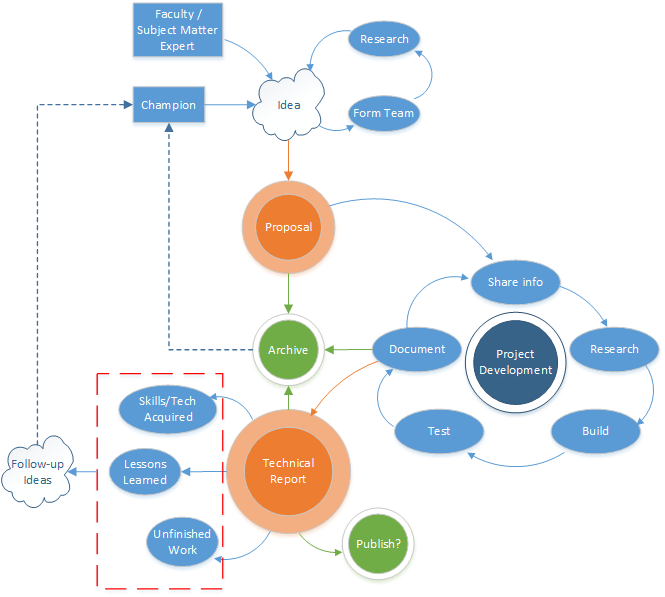
\includegraphics[]{figs/project-life-cycle.png}
%  \caption{Enlarged version of the diagram in \autoref{fig:lifecycle}.}
%\end{figure}

\end{document}
